% R1: robustness (Vaishak). Corruption sweeps (scripts/run_corruption.py), out-of-
% distribution splits (scripts/run_ood.py) and Subspace Alignment (scripts/run_sa.py),
% 5 seeds each; tables and figure from scripts/make_methods_tables.py.

\section{Robustness}\label{sec:robustness}

\subsection{Sensor corruption}

A phone on a motor is not a laboratory accelerometer. We model three failures, each applied to a
whole raw recording before windowing, at levels 0--0.5:
\begin{itemize}
  \item \textbf{Additive noise}: white Gaussian noise with variance equal to the level times
        each channel's vibration variance (level 0.5 is an SNR of 3\,dB).
  \item \textbf{Sample dropout}: a fraction of samples equal to the level is removed in
        contiguous gaps of 5--50 samples, as in Bluetooth packet loss, and filled by linear
        interpolation. A gap removes every channel at once.
  \item \textbf{Gain drift}: each physical axis gets a gain that drifts linearly over the
        recording, $g(t) = 1 + \ell\,(a + (b-a)t/T)$ with $a, b \sim U(-1, 1)$; both channels of
        an axis share it.
\end{itemize}
We test two deployments: the model is trained and tested on corrupted data (the corrupted
signal's own separability), or trained on clean data and tested on corrupted data (a model
deployed on a degraded sensor).

\begin{figure*}[t]
  \centering
  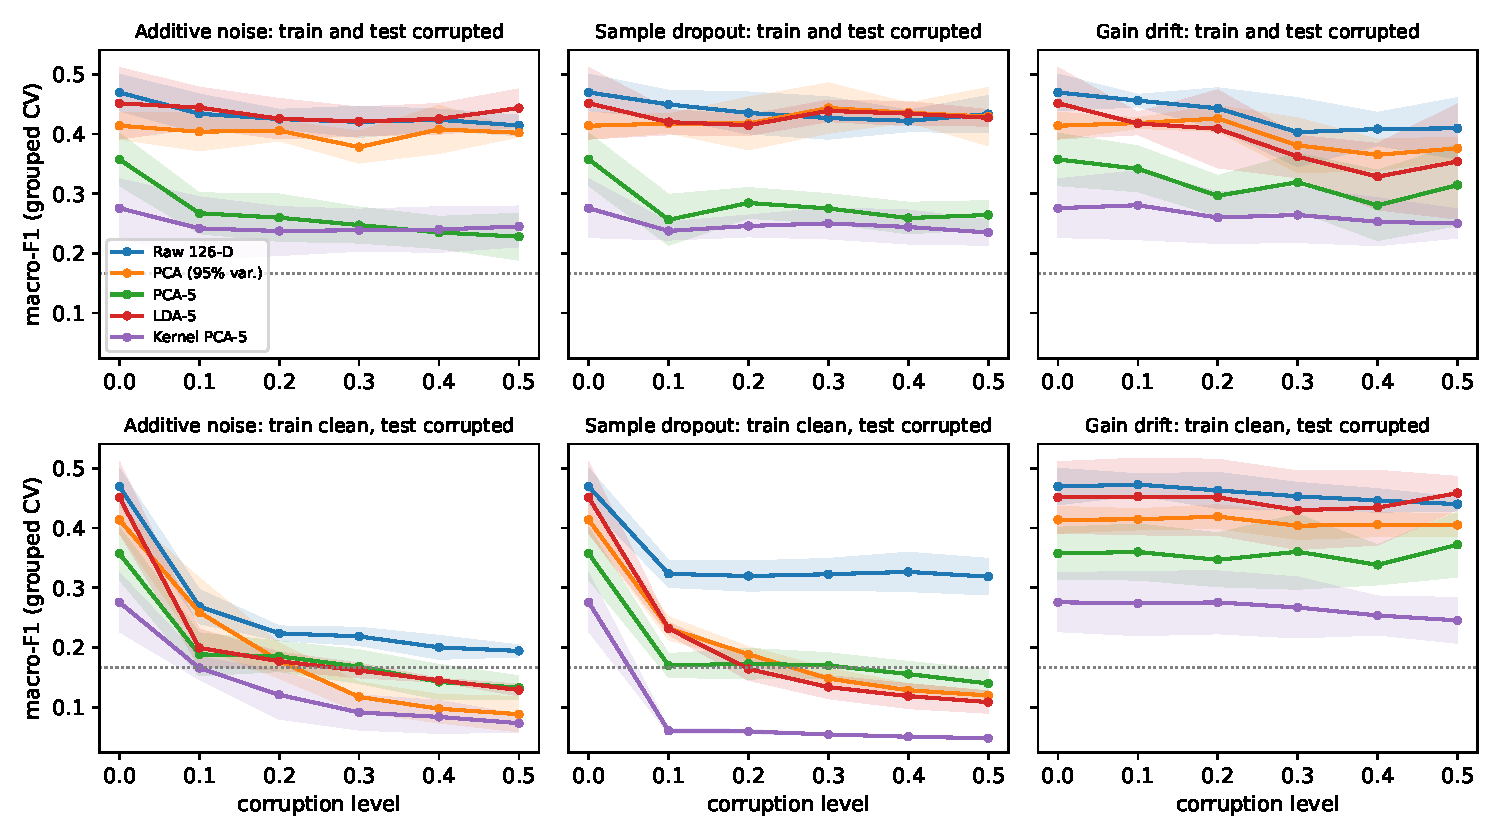
\includegraphics[width=\textwidth]{figures/fig_corruption.pdf}
  \caption{Best macro-F1 per front-end against corruption level (grouped CV, mean $\pm$ 1 std
  over 5 seeds). Top: training and test data corrupted alike. Bottom: clean training data,
  corrupted test data. Dotted line: chance.}
  \label{fig:corruption}
\end{figure*}

The two deployments behave in opposite ways (Fig.~\ref{fig:corruption}). When training and test
data are corrupted alike, noise and dropout barely matter, even at 50\%: the class information
survives and the model adapts to it. Gain drift is the one that hurts, and it hurts LDA most
($0.45 \to 0.35$ at level 0.5), because the per-recording gain breaks the absolute amplitude
cues LDA relies on. When the model is trained on clean data, the picture reverses. Ten percent
noise or dropout already drops every projected front-end to 0.17--0.26, and Kernel PCA to
0.06--0.17. Gain drift barely matters, since most features are scale-free ratios. The raw
features degrade least (0.32 at every dropout level). Noise and dropout therefore do not erase
the classes; they shift the feature distribution (kurtosis, spectral kurtosis and entropy;
interpolation strips high-frequency content), and projections fitted on clean data are the most
brittle to that shift.

\subsection{Unseen operating conditions}

Grouped cross-validation mixes speed and load. To separate them we use two fixed splits: train on
30 and 50\,Hz supply and test on 40\,Hz (both loads), and train unloaded and test loaded (all
speeds).

\begin{table}[t]
  \centering
  \caption{Out-of-distribution splits: best classifier per front-end (macro-F1, mean $\pm$ std
  over 5 seeds).}
  \label{tab:ood}
  \resizebox{\columnwidth}{!}{\begin{tabular}{lcccc}
\toprule
 & \multicolumn{2}{c}{Cross-speed (test 40\,Hz)} & \multicolumn{2}{c}{Cross-load (test loaded)} \\
Front-end & macro-F1 & classifier & macro-F1 & classifier \\
\midrule
Raw 126-D & 0.66 $\pm$ 0.02 & RF & 0.41 $\pm$ 0.02 & RF \\
PCA (95\% var.) & 0.54 $\pm$ 0.03 & RF & 0.15 $\pm$ 0.00 & Lin.\ SVM \\
PCA-5 & 0.52 $\pm$ 0.01 & RF & 0.14 $\pm$ 0.00 & Lin.\ SVM \\
LDA-5 & 0.60 $\pm$ 0.00 & $k$-NN & 0.39 $\pm$ 0.06 & RF \\
Kernel PCA-5 & 0.32 $\pm$ 0.01 & RBF SVM & 0.05 $\pm$ 0.00 & GNB \\
\midrule
\multicolumn{5}{l}{Cross-load recall, Raw 126-D + RF: H 0.64, B1 0.92, B2 0.00, B3 0.26, V 0.68, R 0.16} \\
\bottomrule
\end{tabular}
}
\end{table}

A new speed is easy: the best model reaches $0.66 \pm 0.02$ (Table~\ref{tab:ood}), higher than
grouped cross-validation, because the test speed lies between two training speeds at both loads.
A new load is the hard shift. Loading lowers the shaft speed and raises the slip, which moves the
whole harmonic comb: both linear PCA front-ends fall to 0.14--0.15 and Kernel PCA to 0.05
(one class predicted for almost everything). The raw features and LDA-5 keep about 0.40. Per class, B1 survives the load
change (recall 0.92) while R falls to 0.16 and B2 to 0: R's most consistent signature is its
load-dependent slip (Section~\ref{sec:separability}), and a model that has never seen a loaded
motor cannot use it.

\subsection{Adapting to the new condition}

Subspace Alignment \cite{fernando2013} adapts a model to an unseen condition using its
unlabelled windows: each domain is z-scored with its own statistics and projected onto its own
top-$k$ PCA basis, and the source basis $P_s$ is aligned to the target basis $P_t$ with
$M = P_s^\top P_t$, the least-squares map between them. A classifier trained on
$z_s P_s M$ is applied to $z_t P_t$. We compare it with two controls on the same $k$: no
adaptation (one scaler and PCA fitted on the source, as in every other experiment) and
per-domain z-scoring alone, followed by the source PCA. Targets are each supply frequency in
turn (training on the other two) and the loaded condition.

\begin{table}[t]
  \centering
  \caption{Adapting to an unseen condition: macro-F1 with no adaptation, per-domain z-scoring
  and Subspace Alignment (SA), mean over 5 seeds. Left: best of the six classifiers; right:
  their mean.}
  \label{tab:sa}
  \resizebox{\columnwidth}{!}{\begin{tabular}{llcccccc}
\toprule
 & & \multicolumn{3}{c}{Best classifier} & \multicolumn{3}{c}{Mean of 6 classifiers} \\
Target & $k$ & none & z-score & SA & none & z-score & SA \\
\midrule
Unseen speed (mean of 3) & 5 & 0.31 & 0.46 & 0.46 & 0.25 & 0.39 & 0.34 \\
 & 10 & 0.36 & 0.51 & 0.55 & 0.32 & 0.46 & 0.43 \\
 & 20 & 0.38 & 0.54 & 0.57 & 0.27 & 0.45 & 0.45 \\
Unseen load & 5 & 0.14 & 0.60 & 0.53 & 0.08 & 0.49 & 0.43 \\
 & 10 & 0.18 & 0.42 & 0.48 & 0.08 & 0.37 & 0.38 \\
 & 20 & 0.17 & 0.44 & 0.53 & 0.09 & 0.39 & 0.42 \\
\bottomrule
\end{tabular}
}
\end{table}

Adaptation helps a great deal, most of all for load: from 0.14--0.18 without adaptation to
0.42--0.60 (Table~\ref{tab:sa}). But most of that gain comes from z-scoring each domain with its
own statistics, which re-centres the shifted features. The alignment step adds little on top and
in either direction depending on $k$: for the unseen load it is behind z-scoring at $k=5$ (0.53
against 0.60) and ahead at $k=10$ and 20 (by about 0.06--0.09); averaged over classifiers the two
are within 0.06 of each other everywhere. On this data the condition shift is mostly a change of
location and scale per feature, which per-domain normalisation already corrects. Both adapted
models use the target's unlabelled windows, so they assume access to unlabelled data from the
new condition before deployment.
